\documentclass[letterpaper]{jdf}
\usepackage{etoolbox}
\makeatletter
\patchcmd{\@verbatim}
  {\verbatim@font}
  {\verbatim@font\small}
  {}{}
\makeatother

\pdfstringdefDisableCommands{ \def\\{} }

%\addbibresource{references.bib}

\author{Geoff Scheid}
\email{gscheid3@gatech.edu}
\title{CS 6440 - Intro to Health Informatics:\\Practicum Sprint 2}

\begin{document}

\maketitle

\section{Project Research}
    \subsection{Background}
    Crohn's disease is a chronic inflammatory bowel disease that affects millions of people worldwide.
    It is a condition that causes inflammation and irritation in the digestive tract, 
    leading to symptoms such as abdominal pain, diarrhea, and fatigue. 
    Crohn's disease is a complex condition that can have a significant impact on a person's quality of life, 
    and managing it can be challenging.\\
    Additional information on Crohn's disease my be found here:\\
    https://www.crohnscolitisfoundation.org/what-is-crohns-disease

    \subsection{Justification}
    One way to manage Crohn's disease is by tracking symptoms, 
    which can help patients and healthcare providers better understand the disease and how it is affecting the patient. 
    A web app designed for this purpose can make symptom tracking easier and more convenient for patients, 
    and provide valuable insights into the condition for healthcare providers.\\
    A template symptom tracker provided by the Crohn's and Colitis Foundation:\\
    https://www.crohnscolitisfoundation.org/sites/default/files/legacy/assets/pdfs/ibd-symptom-tracker.pdf

    \subsection{Solution}
    The goal of this project is to create a web app that allows patients with Crohn's disease to easily track their symptoms, 
    monitor their condition over time, and share their symptom data with their healthcare providers. 
    The app will be designed with the patient's needs in mind, with a user-friendly interface and intuitive features. 
    By empowering patients to take a more active role in managing their condition, 
    the app can help improve their quality of life and overall health outcomes.

\section{Technical Design}
    \subsection{Tools/Technology}
    \begin{itemize}
        \item IDE: Visual Studio Code
        \item Programming Languages: HTML, CSS, JavaScript/Typescript
        \item Front-end Library: Bootstrap
        \item Web Development Framework: Angular
        \item Testing Library: Jasmine
        \item Hosting Services: Heroku
        \item Version Control: Git
    \end{itemize}

    \subsection{Data/Data Sources}
    All data will be generated by the patient and will be stored locally only for the length of the browser session.
    To limit the scope of this project, no persistent data storage will be provided.
    No other data sources will be needed for this web app.

    \subsection{Architecture Diagram}
    To limit the scope of this project to the recommended 100 hours, 
    this web app will be a self-contained single page app with no backend, database, or API connections.
    Thus no architectural diagram is required.

    \subsection{Screen Mock-up}
    \begin{jdffigure}
        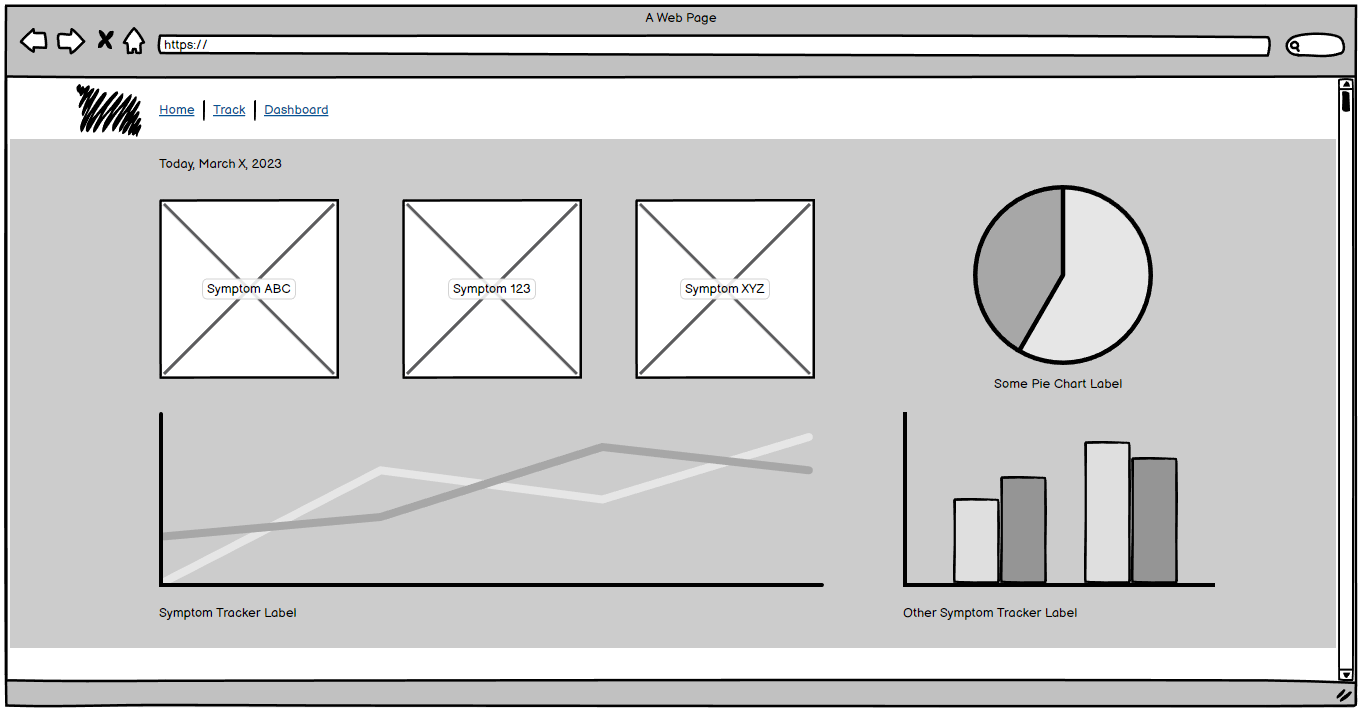
\includegraphics[height=8cm]{Figures/Screen Mockup.PNG}
        \captionof{figure}{Dashboard Screen Mockup}\label{fig:Mockup}
    \end{jdffigure}

\section{Implementation Plan}

    \begin{jdftable}
        \small
        \begin{tabular}{@{} C{0.05\linewidth} L{0.5\linewidth} L{0.2\linewidth}}
            \textbf{Weeks} & \textbf{Project Tasks} & \textbf{Needs/Risks}\\
            \toprule[0.5pt]
            9-10 
            & Design the user interface of the web app using Angular. 
            Implement the front-end components of the web app, including forms for entering symptom data, 
            charts for displaying symptom history, and a dashboard for viewing trends and summaries. 
            & Working with new libraries to display charts/graphs may prove challenging\\
            \midrule
            11-12 
            & Develop the logic for storing and retrieving data from local storage or session storage. 
            & \\
            \midrule
            13 
            & Test the front-end components to ensure that they are working correctly and that data is being stored 
            and retrieved properly. Deploy the front-end application to Heroku. 
            & Need to ensure Heroku account will allow new app.\\
            \midrule
            14 
            & Test and debug the entire web app to ensure that it is functioning correctly 
            and that data is being stored and retrieved properly. 
            & \\
            \midrule
            15 
            & Create final delivery documentation and instructions for using the web app and submit project. 
            & \\
        \end{tabular}
        \captionof{table}{Practicum Implementation Plan}\label{table:Plan}
    \end{jdftable}

\end{document}